\section{Obtención de conjunto de datos}


La obtención del conjunto de datos se divide en dos etapas, la primera es la toma de muestras, la cual implica ir al lugar con flujo constante de vehículos para obtener la mayor cantidad de estos en el menor tiempo posible, y la segunda etapa es la limpieza de las muestras con la cual se busca solo tomar en cuenta los vehículos a los que se logro tomar correctamente la velocidad.
La Figura \ref{fig:DFCreacionCD} muestra las dos etapas internas con las que cuenta la obtención de conjunto de datos.

\begin{figure}[H]
    \centering
    \begin{tikzpicture}

        \node(a0)[rectangle,
            draw=black,
            minimum width=7cm,
            minimum height=3.6cm,
            label=Obtención de conjunto de datos]
            {};

        \node(a)[rectangle, draw=black, minimum width=5cm, minimum height=1cm] at ([yshift=-2em]a0.north)
        % [inside=of a0]
            {Toma de muestras};

        \node(b)[rectangle, draw=black, minimum width=5cm, minimum height=1cm]
            [below=of a]
            {Limpieza de las muestras};

        \draw[->] (a) -- (b);

    \end{tikzpicture}

    \caption{Proceso de obtención de conjunto de datos.}
    \label{fig:DFCreacionCD}
\end{figure}


% El diagrama de flujo de la Figura \ref{fig:DFCreacionCD} muestra el proceso completo para generar un conjunto de datos, en este vemos que una vez que se toman todas las muestras los tres siguientes pasos son iterativos hasta que las hayamos procesado todas.


%%%%%%%%%%%%%%%%%%%%%%%%%%%%%%%%%%%%%%%%%%%%%%%%%%%%%%%%%%%%%%%%%%%%%%%%%%%%%%%%
%%%%%%%%%%%%%%%%%%%%%%%%%%%%%%%%%%%%%%%%%%%%%%%%%%%%%%%%%%%%%%%%%%%%%%%%%%%%%%%%
%%%%%%%%%%%%%%%%%%%%%%%%%%%%%%%%%%%%%%%%%%%%%%%%%%%%%%%%%%%%%%%%%%%%%%%%%%%%%%%%
%%%%%%%%%%%%%%%%%%%%%%%%%%%%%%%%%%%%%%%%%%%%%%%%%%%%%%%%%%%%%%%%%%%%%%%%%%%%%%%%
%%%%%%%%%%%%%%%%%%%%%%%%%%%%%%%%%%%%%%%%%%%%%%%%%%%%%%%%%%%%%%%%%%%%%%%%%%%%%%%%

\subsection{Toma de muestras}

Para la toma de muestras se requirió de dos dispositivos con los cuales se busca la extracción de conjunto de datos que posteriormente se utilizara como entrenamiento de los modelos predictivos. Uno de los dispositivos es el radar Bushnell (Figura \ref{fig:RadarVelocidad}) con una precisión de +/- 1.6 kilómetros por hora.

\begin{figure}[H]
    \centering
    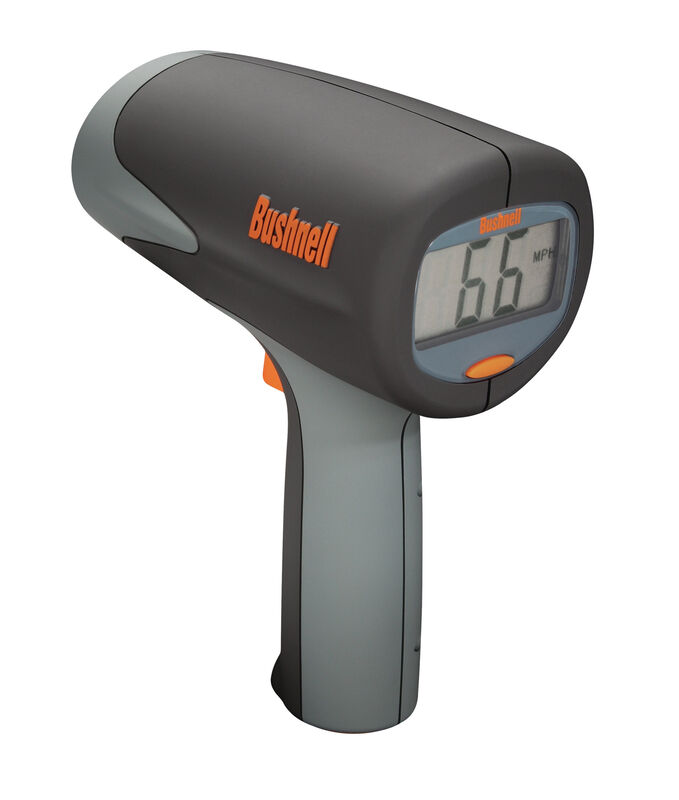
\includegraphics[width=0.4\textwidth]{Metodologia/imgs/bushnell.jpg}
    \caption{Radar de velocidad Bushnell.}
    \label{fig:RadarVelocidad}
\end{figure}

Mientras que el otro dispositivo es una cámara de video, la cual puede ser un dispositivo especializado para esta tarea o cualquier otro dispositivo capaz de grabar video. Las configuraciones mínimas pueden ser una resolución de 854 x 480 a 30 fotogramas por segundo, sin embargo, hay que tomar en cuenta que al tener una resolución tan baja podemos perder calidad en la imagen y tomar un área menor a la deseada, mientras que tener fotogramas tan bajos nos ocasionaría perder vehículo que pasan a una velocidad más alta. Por otro parte al aumentar la resolución y los fotogramas por segundo estamos ocasionando que al sistema le tome más tiempo procesarlos. Para este caso se utilizó la cámara de Smartphones un Xiaomi Redmi Note 7 y un iPhone X configurados a 60 FPS y una resolución de Full HD (1920 x 1080 pixeles).

Se tomo especial cuidado a la hora de posicionar la cámara, ya que no se quiere que los experimentos sean considerados como cálculos de velocidad en 2D, para esto la toma de muestras se realizó en un lugar donde el tráfico vehicular pase con cierto grado de inclinación, sin apuntar la cámara directamente al costado de donde pasan los vehículos, como muestra la Figura \ref{fig:LugarMuestrasDataset}.

\begin{figure}[H]
    \centering
    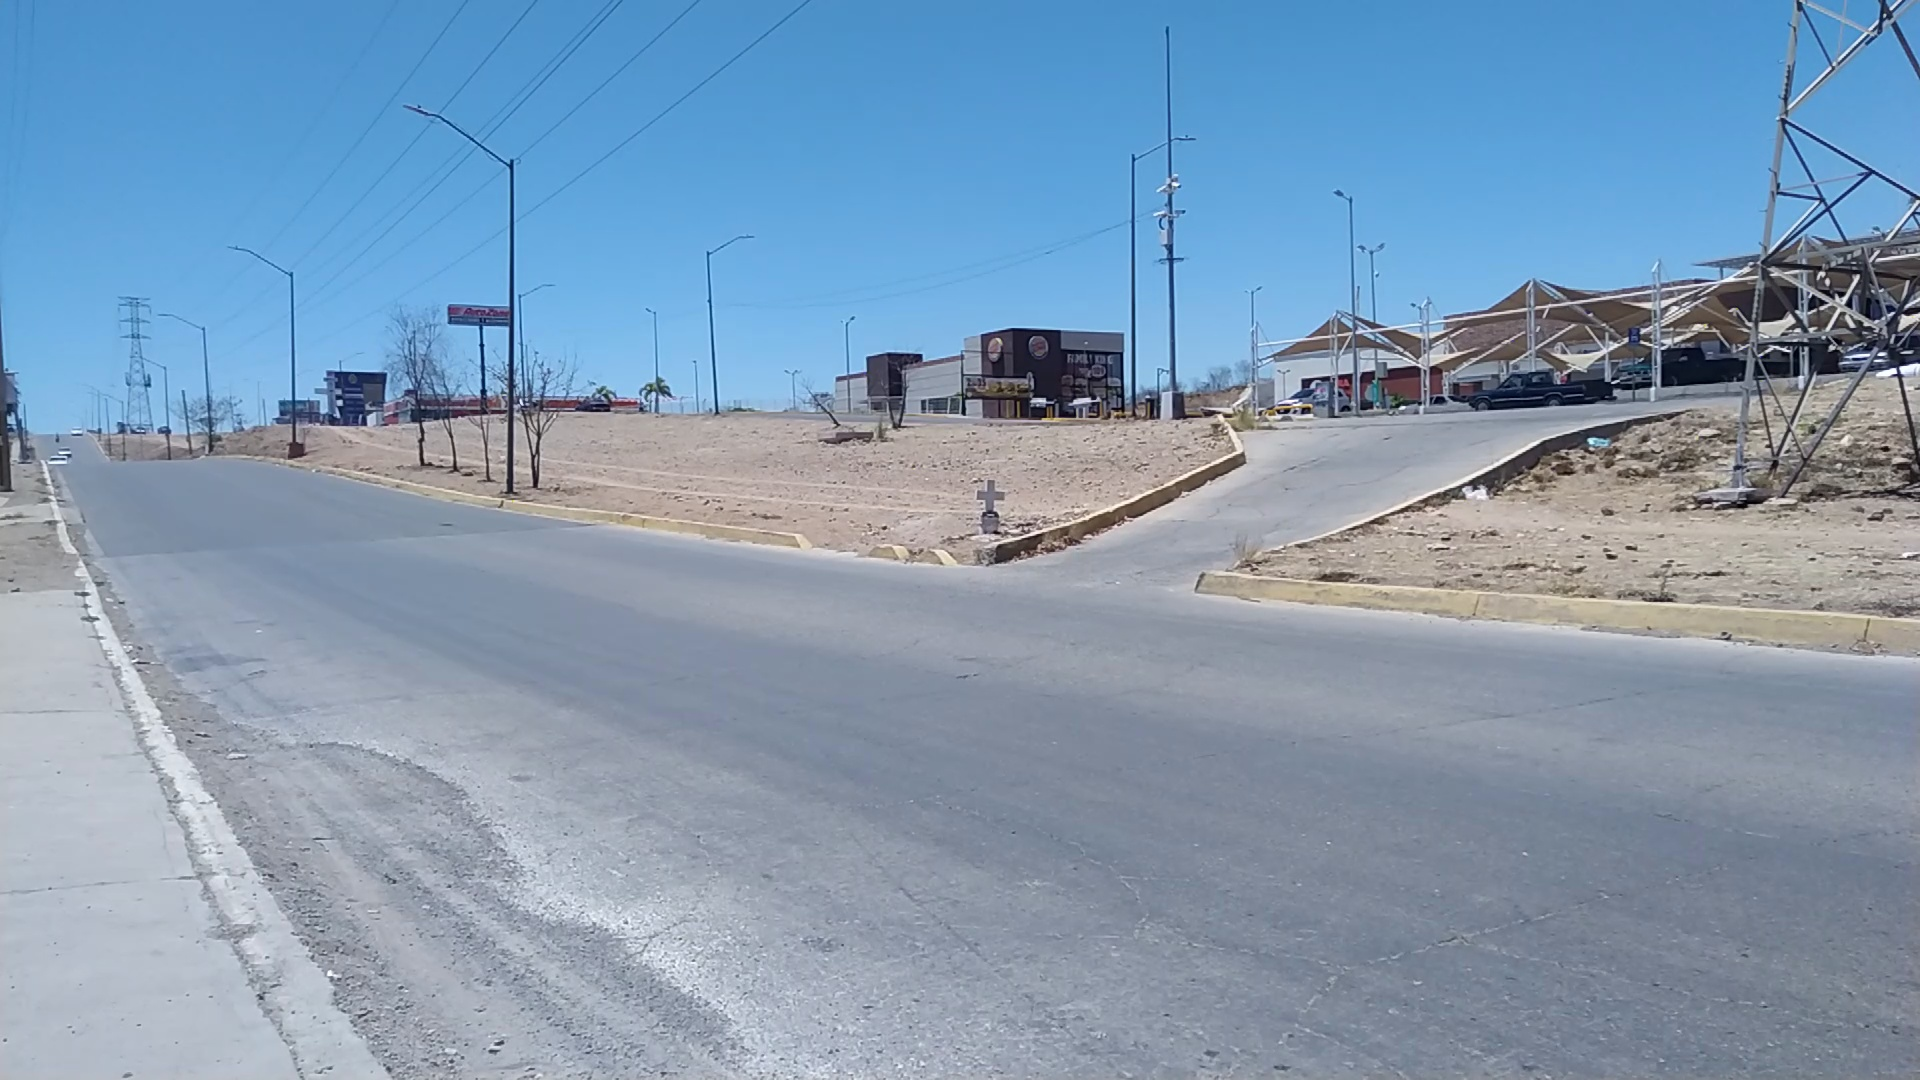
\includegraphics[width=0.8\textwidth]{Metodologia/imgs/LugarMuestras.jpg}
    \caption{Lugar donde se tomaron las muestras.}
    \label{fig:LugarMuestrasDataset}
\end{figure}

Cabe mencionar que para hacer más practica y rápido la toma de muestras, estas fueron tomadas en este mismo lugar, en la ciudad de Culiacán, Sinaloa.

Dado que la cámara y el radar de velocidad son dispositivos que no están sincronizados entre si para darnos el video y la velocidad, nos aseguramos se guardar la velocidad detectada por el radar en el video tomada, diciéndola en voz alta al micrófono de la cámara.

%%%%%%%%%%%%%%%%%%%%%%%%%%%%%%%%%%%%%%%%%%%%%%%%%%%%%%%%%%%%%%%%%%%%%%%%%%%%%%%%
%%%%%%%%%%%%%%%%%%%%%%%%%%%%%%%%%%%%%%%%%%%%%%%%%%%%%%%%%%%%%%%%%%%%%%%%%%%%%%%%
%%%%%%%%%%%%%%%%%%%%%%%%%%%%%%%%%%%%%%%%%%%%%%%%%%%%%%%%%%%%%%%%%%%%%%%%%%%%%%%%
%%%%%%%%%%%%%%%%%%%%%%%%%%%%%%%%%%%%%%%%%%%%%%%%%%%%%%%%%%%%%%%%%%%%%%%%%%%%%%%%
%%%%%%%%%%%%%%%%%%%%%%%%%%%%%%%%%%%%%%%%%%%%%%%%%%%%%%%%%%%%%%%%%%%%%%%%%%%%%%%%

\subsection{Limpieza de las muestras}

Una vez tomadas las muestras es necesario realizar una limpieza de los datos, estos son, los vehículos a los que se les tomo la velocidad utilizando el radar. Ya que el video y el radar no están sincronizados por hardware es necesario realizar una inspección visual de las muestras.

Considerando que la cámara de video y el radar no son dispositivos especializados para esta tarea, fue necesario definir una manera de unir los datos del video con la velocidad, así que se implementó el sistema pensando en que recibiría como entrada un archivo CSV con el mismo nombre que la muestra, pero con la extensión TXT. Este archivo contiene los datos necesarios para realizar la unión de las características del video y la velocidad, los valores del archivo son los siguientes:

\begin{itemize}
    \item Segundo en que pasa el vehículo
    \item Velocidad detectada por el radar
    \item Carril
    \item Descripción del vehículo
\end{itemize}

Para poder determinar la velocidad siempre es necesario tomar el tiempo que le toma a un objeto pasar de un lugar a otro, para esto el sistema necesita ser configurado con un punto de entrada y un punto de salida en el eje X, para fines prácticos a partir de ahora llamaremos a estos dos puntos simplemente punto A y punto B.  Estos dos puntos deben ser colocados de manera que los vehículos deben pasar completamente por cada uno de ellos, además que cada una de las muestras pueden tener diferentes valores para los puntos A y B, sin embargo, para nuestro caso no fue necesario implementar diferentes valores ya que todos los videos fueron tomados en el mismo lugar. La Figura \ref{fig:LugarLimites} muestras donde fueron colocados los puntos A y B en nuestras muestras.

\begin{figure}[H]
    \centering
    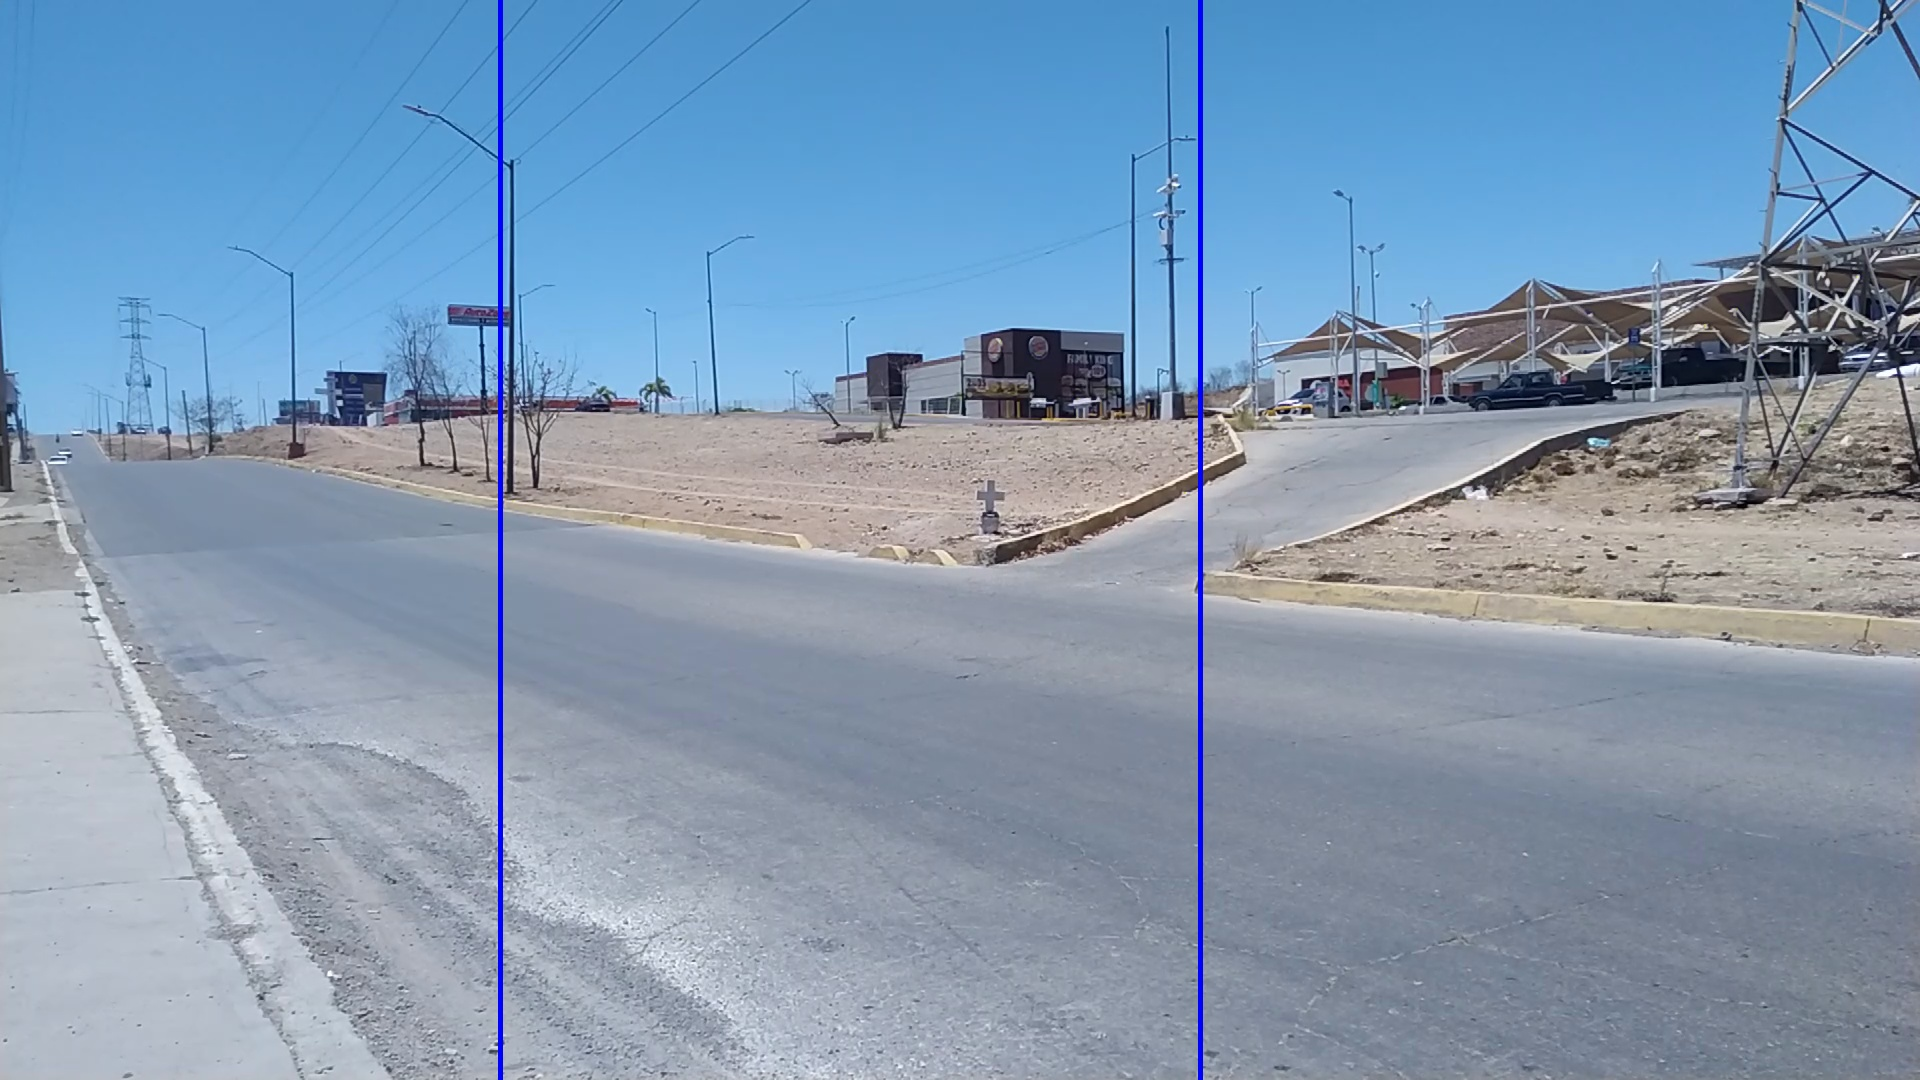
\includegraphics[width=0.8\textwidth]{Metodologia/imgs/LugarLimites.jpg}
    \caption{Limites para lugar de las muestras.}
    \label{fig:LugarLimites}
\end{figure}

Una vez que tenemos los valores para los puntos A y B podemos comenzar a generar el archivo CVS, para esto debemos tomar en cuenta que el segundo en que pasa debe ser lo más cercano posible al centroide del vehículo cuando pasa por el punto B, es importante ingresar una descripción, aunque esta no va a ser usada por el sistema, se volverá importante para validar que el vehículo al que se le tomo la velocidad es el mismo que detecto el sistema.

%%%%%%%%%%%%%%%%%%%%%%%%%%%%%%%%%%%%%%%%%%%%%%%%%%%%%%%%%%%%%%%%%%%%%%%%%%%%%%%%
%%%%%%%%%%%%%%%%%%%%%%%%%%%%%%%%%%%%%%%%%%%%%%%%%%%%%%%%%%%%%%%%%%%%%%%%%%%%%%%%
%%%%%%%%%%%%%%%%%%%%%%%%%%%%%%%%%%%%%%%%%%%%%%%%%%%%%%%%%%%%%%%%%%%%%%%%%%%%%%%%
%%%%%%%%%%%%%%%%%%%%%%%%%%%%%%%%%%%%%%%%%%%%%%%%%%%%%%%%%%%%%%%%%%%%%%%%%%%%%%%%
%%%%%%%%%%%%%%%%%%%%%%%%%%%%%%%%%%%%%%%%%%%%%%%%%%%%%%%%%%%%%%%%%%%%%%%%%%%%%%%%
